Given X and Y are two continuous random variables with joint probability density function,
\begin{align}
f\brak{x,y}= 
\begin{cases}
ae^{-2y} & 0<x<y<\infty \\
0 & \text{otherwise}.
\end{cases}   
\end{align}
% \begin{figure}[!hbt]
%     \centering
%     \includegraphics[width=\columnwidth]{Figure_0.png}
%     \caption{Graph of x=y}
%     \label{Figure_1}
% \end{figure}
We know that,\\
$0<x<y<\infty  \implies x<y<\infty \text{ for } 0<x<\infty.$\\ 
Then,
\begin{align}
    f_X\brak{x} &= \int f_{XY}\brak{x,y}dy\\
    &= \int_{x}^{\infty} ae^{-2y}dy\\
    &= \left[ \frac{ae^{-2y}}{(-2)} \right]_{x}^{\infty}\\
    &= \frac{-a}{2}\left[ e^{-2y}\right]_{x}^{\infty}\\
    &= \frac{-a}{2}[0-e^{-2x}]\\
\implies f_X\brak{x} &=
    \begin{cases}
    \frac{a}{2}e^{-2x} & 0 < x < \infty\\
    0 & \text{otherwise}.
    \end{cases}
\end{align}
Similarly,\\
$ 0<x<y<\infty \implies 0<x<y \text{ for } 0<y<\infty$ \\
Then,
\begin{align}
    f_y\brak{y} &= \int f_{XY}\brak{x,y}dx\\
    &= \int_{0}^{y} ae^{-2y}dx\\
    &= ae^{-2y}[x]_{0}^{y}\\
    &= aye^{-2y}\\
\implies f_Y\brak{y} &=
    \begin{cases}
    aye^{-2y} & 0 < y < \infty\\
    0 & \text{otherwise}.
    \end{cases}
\end{align}
%\begin{figure}[ht]
%    \centering
%    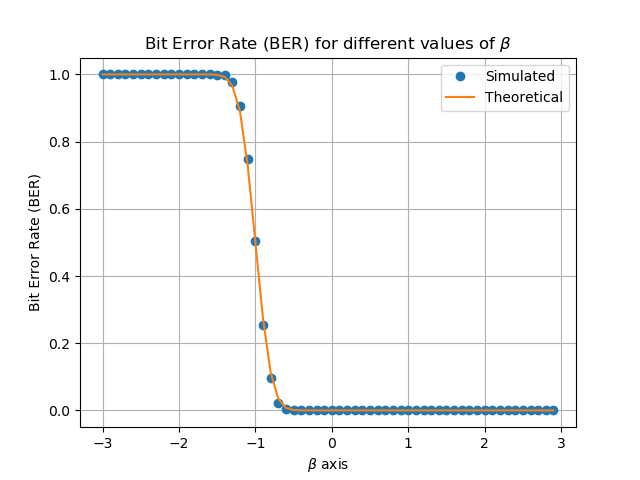
\includegraphics[width=\columnwidth]{Figure_1.png}
%    \caption{Graph of x+y=1}
%    \label{Figure_1}
%\end{figure}
Therefore ,
\begin{align}
    f_{X|Y}\brak{x|y} &= \frac{f_{XY}\brak{x,y}}{f_Y\brak{y}}\\
    & = \frac{ae^{-2y}}{aye^{-2y}}\\
    & = \frac{1}{y}\\
\implies f_{X|Y}\brak{x|y} &=
    \begin{cases}
    \frac{1}{y} & \text{if } 0<x<y<\infty\\
    0 & \text{otherwise}
    \end{cases}
\end{align}
Then, 
\begin{align}
   E\brak{X|Y=y} & =
   \int_{-\infty}^{\infty} (x)f_{X|Y}\brak{x|y}dx\\
    & = \int_{0}^{y}(x)\brak{\frac{1}{y}}dx\\
    & = \frac{1}{y} \int_{0}^{y}(x)dx \\
    & = \frac{1}{y} \left[ \frac{x^2}{2}\right]_{0}^{y}\\
    & = \frac{1}{y}\brak{\frac{y^2}{2}}\\
    & = \frac{y}{2}\\
\implies E\brak{X|Y=y} &= \frac{y}{2}\\
\therefore E\brak{X|Y=2} &= 1
\end{align}